\documentclass[aspectratio=169]{beamer}
\usetheme{Madrid}
\usecolortheme{default}

% Packages
\usepackage[utf8]{inputenc}
\usepackage[T1]{fontenc}
\usepackage{amsmath,amssymb}
\usepackage{graphicx}
\usepackage{booktabs}
\usepackage{tikz}
\usetikzlibrary{shapes,arrows,positioning}
\usepackage{algorithm}
\usepackage{algorithmic}
\usepackage{colortbl}

% Title information
\title[Optimizing LMs for Domain-Specific Tasks]{Optimizing and Adapting Language Models \\ for Domain-Specific Tasks}
\subtitle{Advanced RAG \& Parameter-Efficient Fine-Tuning}
\author{Minh Duy Nguyen}
\institute{Torus AI \\ Supervised by: [Supervisor Names]}
\date{\today}

% Custom colors
\definecolor{torusblue}{RGB}{0,102,204}
\definecolor{torusgreen}{RGB}{34,139,34}
\definecolor{torusred}{RGB}{204,0,0}

\begin{document}

% ====================
% SLIDE 1: Title
% ====================
\begin{frame}
\titlepage
\end{frame}

% ====================
% SLIDE 2: Motivation & Problem Statement
% ====================
\begin{frame}{Motivation \& Problem Statement}
\begin{block}{Enterprise Challenges in LLM Deployment}
Two fundamental gaps when deploying Generative AI:
\end{block}

\begin{columns}[T]
\column{0.48\textwidth}
\begin{alertblock}{Knowledge Gap}
\begin{itemize}
    \item Static training data
    \item Hallucination risks
    \item No access to proprietary documents
\end{itemize}
\end{alertblock}

\column{0.48\textwidth}
\begin{alertblock}{Behavior Gap}
\begin{itemize}
    \item Inconsistent communication style
    \item Cannot follow domain workflows
    \item Out-of-character drift
\end{itemize}
\end{alertblock}
\end{columns}

\vspace{0.5cm}
\begin{center}
\textbf{How can we bridge these gaps with resource-constrained deployment?}
\end{center}
\end{frame}

% ====================
% SLIDE 3: Report Overview
% ====================
\begin{frame}{Report Overview}
\begin{center}
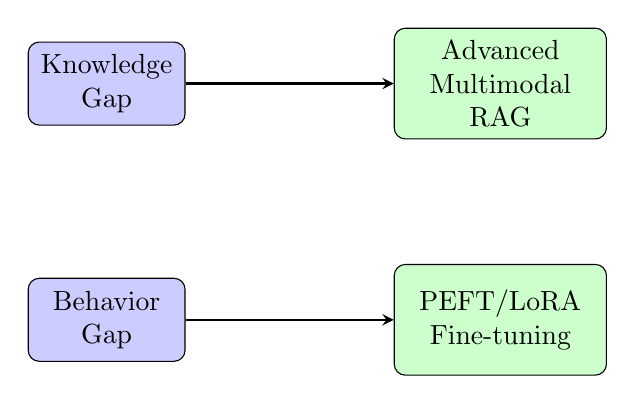
\begin{tikzpicture}[node distance=2cm, auto]
    % Styles
    \tikzstyle{block} = [rectangle, draw, fill=blue!20, text width=5em, text centered, rounded corners, minimum height=3em]
    \tikzstyle{solution} = [rectangle, draw, fill=green!20, text width=7em, text centered, rounded corners, minimum height=4em]
    \tikzstyle{arrow} = [thick,->,>=stealth]
    
    % Nodes
    \node [block] (kg) {Knowledge Gap};
    \node [block, below of=kg, node distance=3cm] (bg) {Behavior Gap};
    \node [solution, right of=kg, node distance=5cm] (rag) {Advanced \\ Multimodal RAG};
    \node [solution, right of=bg, node distance=5cm] (peft) {PEFT/LoRA \\ Fine-tuning};
    
    % Arrows
    \draw [arrow] (kg) -- (rag);
    \draw [arrow] (bg) -- (peft);
\end{tikzpicture}
\end{center}

\begin{block}{Two Complementary Solutions}
\begin{itemize}
    \item \textbf{RAG Pipeline:} Accurate retrieval from complex documents (text, tables, images)
    \item \textbf{Fine-tuned SLMs:} Behavioral consistency at low cost
\end{itemize}
\end{block}
\end{frame}

% ====================
% BLOCK A: RAG
% ====================

% ====================
% SLIDE 4: RAG Background
% ====================
\begin{frame}{RAG Background: Basic Pipeline}
\begin{columns}[T]
\column{0.5\textwidth}
\textbf{Indexing Phase (Offline)}
\begin{enumerate}
    \item Document Loading
    \item Chunking
    \item Embedding
    \item Vector Storage
\end{enumerate}

\column{0.5\textwidth}
\textbf{Query Phase (Online)}
\begin{enumerate}
    \item Query embedding
    \item Similarity search
    \item Context augmentation
    \item LLM generation
\end{enumerate}
\end{columns}

\vspace{0.5cm}
\begin{center}
\textit{Standard approach: Dense retrieval with simple text chunking}
\end{center}
\end{frame}

% ====================
% SLIDE 5: Limitations of Simple RAG
% ====================
\begin{frame}{Limitations of Simple RAG}
\begin{alertblock}{Three Critical Issues}
\begin{enumerate}
    \item \textbf{Structure Loss:} Tables and layouts destroyed during parsing
    \begin{itemize}
        \item Financial reports, medical forms become unreadable
    \end{itemize}
    
    \item \textbf{Monolingual Bias:} MiniLM optimized for English
    \begin{itemize}
        \item Poor performance on French documents (GPM use case)
    \end{itemize}
    
    \item \textbf{"Lost in the Middle":} LLMs struggle with long contexts
    \begin{itemize}
        \item Relevant info buried in retrieved chunks
    \end{itemize}
\end{enumerate}
\end{alertblock}

\vspace{0.3cm}
\begin{center}
\textcolor{torusred}{\textbf{Simple RAG: 0.648 correctness, 0.654 context precision}}
\end{center}
\end{frame}

% ====================
% SLIDE 6: Advanced RAG Architecture
% ====================
\begin{frame}{Advanced RAG: Three-Pillar Architecture}
\begin{block}{Three-Pillar Design}
\begin{enumerate}
    \item \textbf{Structure Preservation}
    \begin{itemize}
        \item UnstructuredIO: Maintains table structure, extracts images
    \end{itemize}
    
    \item \textbf{Semantic Enrichment}
    \begin{itemize}
        \item Multimodal summarization (text + tables + images)
        \item Store both raw + summarized content
    \end{itemize}
    
    \item \textbf{Multi-layer Retrieval}
    \begin{itemize}
        \item Hybrid Search: BM25 (keyword) + Dense (semantic)
        \item Cross-Encoder Reranking: Prevent "Lost in the Middle"
    \end{itemize}
\end{enumerate}
\end{block}

\vspace{0.2cm}
\begin{center}
\textbf{Embedding:} multilingual-e5-large-instruct (best French performance < 1B params)
\end{center}
\end{frame}

% ====================
% SLIDE 7: Use Cases
% ====================
\begin{frame}{Real-World Use Cases}
\begin{columns}[T]
\column{0.48\textwidth}
\begin{block}{GPM Financial Reports}
\textbf{Challenge:}
\begin{itemize}
    \item Complex tables with nested structure
    \item French language documents
    \item Multi-page financial statements
\end{itemize}

\textbf{Task:}
\begin{itemize}
    \item Extract specific figures
    \item Answer accounting queries
\end{itemize}
\end{block}

\column{0.48\textwidth}
\begin{block}{CCAM Medical Coding}
\textbf{Challenge:}
\begin{itemize}
    \item 9,000+ medical procedure codes
    \item Precise code retrieval required
    \item Clinical terminology
\end{itemize}

\textbf{Task:}
\begin{itemize}
    \item Find correct CCAM code
    \item Provide code descriptions
\end{itemize}
\end{block}
\end{columns}
\end{frame}

% ====================
% SLIDE 8: Evaluation Framework
% ====================
\begin{frame}{Evaluation Framework: RAGAS Metrics}
\begin{block}{LLM-as-a-Judge Methodology}
Two judge models: \texttt{gemma-3-12b-it}, \texttt{mistral-small-24b-instruct-2501}
\end{block}

\begin{table}
\centering
\small
\begin{tabular}{ll}
\toprule
\textbf{Metric} & \textbf{Definition} \\
\midrule
Answer Correctness & Semantic similarity: generated vs ground-truth \\
Answer Relevancy & How well response addresses query \\
Faithfulness & Response grounded in retrieved context \\
Context Precision & Relevant chunks ranked highly \\
\midrule
\textbf{Domain-Specific} & \\
Code Hit Rate@k & Correct code in top-k results (CCAM) \\
\bottomrule
\end{tabular}
\end{table}

\vspace{0.2cm}
\textit{All metrics: continuous scale [0, 1], averaged across two judges}
\end{frame}

% ====================
% SLIDE 9: RAG Results
% ====================
\begin{frame}{RAG Evaluation Results}
\begin{columns}[T]
\column{0.48\textwidth}
\begin{table}
\centering
\caption{GPM Test Set (25 questions)}
\scriptsize
\begin{tabular}{lcc}
\toprule
\textbf{Metric} & \textbf{Simple} & \textbf{Advanced} \\
\midrule
Correctness & 0.648 & \textcolor{torusgreen}{\textbf{0.976}} \\
Relevancy & 0.788 & \textcolor{torusgreen}{\textbf{0.972}} \\
Faithfulness & 0.732 & \textcolor{torusgreen}{\textbf{0.940}} \\
Context Prec. & 0.654 & \textcolor{torusgreen}{\textbf{0.960}} \\
\midrule
Improvement & — & \textcolor{torusgreen}{\textbf{+32.8\%}} \\
\bottomrule
\end{tabular}
\end{table}

\column{0.48\textwidth}
\begin{table}
\centering
\caption{CCAM Test Set (10 scenarios)}
\scriptsize
\begin{tabular}{lcc}
\toprule
\textbf{Metric} & \textbf{Simple} & \textbf{Advanced} \\
\midrule
Hit Rate@5 & 0.4 & \textcolor{torusgreen}{\textbf{0.8}} \\
Hit Rate@20 & 0.6 & \textcolor{torusgreen}{\textbf{0.9}} \\
\midrule
Improvement & — & \textcolor{torusgreen}{\textbf{+40\%}} \\
\bottomrule
\end{tabular}
\end{table}
\end{columns}

\vspace{0.5cm}
\begin{block}{Key Takeaway}
Structure preservation + reranking mechanism → \textbf{32.8\% correctness gain}
\end{block}
\end{frame}

% ====================
% BLOCK B: Fine-tuning
% ====================

% ====================
% SLIDE 10: Why Not Prompt Engineering?
% ====================
\begin{frame}{Why Not Just Prompt Engineering?}
\begin{alertblock}{Limitations of In-Context Learning}
\begin{enumerate}
    \item \textbf{Attention Dilution:} Long system prompts → degraded performance
    \item \textbf{Inconsistency:} Out-of-character drift in extended conversations
    \item \textbf{Cost:} Large models (GPT-4) expensive for continuous deployment
\end{enumerate}
\end{alertblock}

\vspace{0.3cm}
\begin{block}{Theoretical Foundation: Intrinsic Dimensionality}
\begin{itemize}
    \item Behavioral patterns lie in a \textbf{low-dimensional subspace}
    \item Parameter-efficient methods (LoRA) can capture this subspace
    \item Small models sufficient to \textbf{reproduce} expert behavior
\end{itemize}
\end{block}

\vspace{0.3cm}
\begin{center}
\textit{"Behavioral expertise is compressible"}
\end{center}
\end{frame}

% ====================
% SLIDE 11: LoRA Theory
% ====================
\begin{frame}{LoRA \& PEFT Theory}
\begin{block}{Low-Rank Adaptation (LoRA)}
Inject trainable low-rank matrices into frozen model:
\[
W' = W_{\text{frozen}} + \underbrace{B A}_{\text{trainable}}
\]
where $W \in \mathbb{R}^{d \times k}$, $B \in \mathbb{R}^{d \times r}$, $A \in \mathbb{R}^{r \times k}$, and $r \ll \min(d, k)$
\end{block}

\begin{columns}[T]
\column{0.48\textwidth}
\textbf{Parameter Count:}
\begin{itemize}
    \item Full FT: Update all $d \times k$ params
    \item LoRA: Only $r(d + k)$ params
    \item Typical: $r = 16$, reduction $\sim$99\%
\end{itemize}

\column{0.48\textwidth}
\textbf{Our Configuration:}
\begin{itemize}
    \item Rank $r = 16$
    \item Applied to: Attention \textbf{+ FFN} layers
    \item Hypothesis: Behavior requires both "seeing" and "processing"
\end{itemize}
\end{columns}
\end{frame}

% ====================
% SLIDE 12: Knowledge Distillation Pipeline
% ====================
\begin{frame}{Knowledge Distillation Pipeline}
\begin{center}
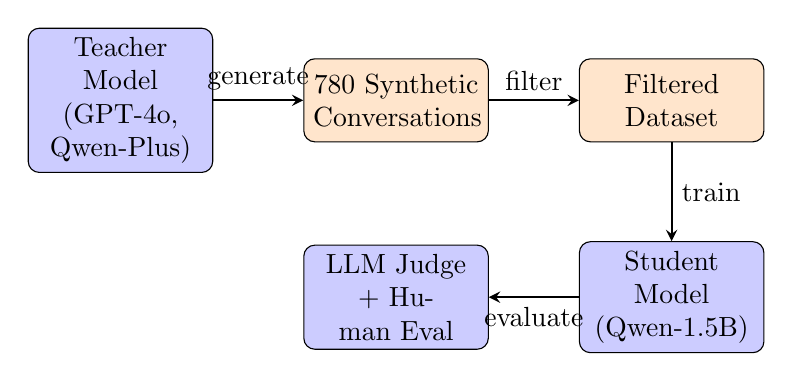
\begin{tikzpicture}[node distance=2.5cm, auto]
    \tikzstyle{process} = [rectangle, draw, fill=blue!20, text width=6em, text centered, rounded corners, minimum height=3em]
    \tikzstyle{data} = [rectangle, draw, fill=orange!20, text width=6em, text centered, rounded corners, minimum height=3em]
    \tikzstyle{arrow} = [thick,->,>=stealth]
    
    \node [process] (teacher) {Teacher Model \\ (GPT-4o, Qwen-Plus)};
    \node [data, right of=teacher, node distance=3.5cm] (synthetic) {780 Synthetic \\ Conversations};
    \node [data, right of=synthetic, node distance=3.5cm] (filtered) {Filtered \\ Dataset};
    \node [process, below of=filtered, node distance=2.5cm] (student) {Student Model \\ (Qwen-1.5B)};
    \node [process, left of=student, node distance=3.5cm] (eval) {LLM Judge \\ + Human Eval};
    
    \draw [arrow] (teacher) -- node[above] {generate} (synthetic);
    \draw [arrow] (synthetic) -- node[above] {filter} (filtered);
    \draw [arrow] (filtered) -- node[right] {train} (student);
    \draw [arrow] (student) -- node[below] {evaluate} (eval);
\end{tikzpicture}
\end{center}

\begin{block}{Three-Stage Process}
\begin{enumerate}
    \item \textbf{Generation:} Teacher models create expert conversations
    \item \textbf{Training:} Student learns behavioral patterns via supervised fine-tuning
    \item \textbf{Evaluation:} Multi-dimensional assessment (LLM + Human)
\end{enumerate}
\end{block}
\end{frame}

% ====================
% SLIDE 13: Case Study - Tarot Reader
% ====================
\begin{frame}{Case Study: Tarot Reader Chatbot}
\begin{columns}[T]
\column{0.55\textwidth}
\begin{block}{Three-Layer Complexity}
\begin{enumerate}
    \item \textbf{Knowledge Layer}
    \begin{itemize}
        \item 78 cards (upright + reversed)
    \end{itemize}
    
    \item \textbf{Operational Layer}
    \begin{itemize}
        \item Ritual workflow: Greeting → Explore → Draw → Interpret → Synthesize
    \end{itemize}
    
    \item \textbf{Emotional Layer}
    \begin{itemize}
        \item Empathetic language
        \item Open-ended questions
        \item Maintain character consistency
    \end{itemize}
\end{enumerate}
\end{block}

\column{0.4\textwidth}
\begin{center}
\fbox{\parbox{0.9\textwidth}{
\centering
\textit{[Demo Screenshot]} \\
\vspace{2cm}
\small User draws 3 cards, \\
receives personalized reading
}}
\end{center}
\end{columns}

\vspace{0.3cm}
\textbf{Why good test bed?} Behavioral complexity $>>$ knowledge complexity
\end{frame}

% ====================
% SLIDE 14: Model Selection
% ====================
\begin{frame}{Model Selection \& Training Configuration}
\begin{table}
\centering
\caption{Performance on Standard Benchmarks}
\scriptsize
\begin{tabular}{lccc}
\toprule
\textbf{Model} & \textbf{MMLU} & \textbf{GSM8K} & \textbf{MATH} \\
 & (Knowledge) & (Reasoning) & (Hard Logic) \\
\midrule
Llama-3.2-1B-Instruct & 49.3 & 44.4 & 30.6 \\
Gemma-2-2.6B-Base & 52.2 & 30.3 & 25.3 \\
Qwen2.5-0.5B-Instruct & 47.5 & 49.6 & 34.4 \\
\rowcolor{green!20}
Qwen2.5-1.5B-Instruct & \textbf{60.9} & \textbf{73.2} & \textbf{55.2} \\
\bottomrule
\end{tabular}
\end{table}

\vspace{0.3cm}
\begin{columns}[T]
\column{0.48\textwidth}
\textbf{Why Qwen2.5?}
\begin{itemize}
    \item Best performance/parameter ratio
    \item Strong multilingual capability
    \item Apache 2.0 license
\end{itemize}

\column{0.48\textwidth}
\textbf{LoRA Configuration:}
\begin{itemize}
    \item Rank: 16
    \item Target: Attention + FFN
    \item Trainable params: 1.2\% of total
\end{itemize}
\end{columns}
\end{frame}

% ====================
% SLIDE 15: Fine-tuning Results
% ====================
\begin{frame}{Fine-tuning Results}
\begin{columns}[T]
\column{0.48\textwidth}
\begin{table}
\centering
\caption{LLM-as-a-Judge Scores}
\scriptsize
\begin{tabular}{lcc}
\toprule
\textbf{Model} & \textbf{Avg Score} & \textbf{Win Rate} \\
\midrule
GPT-4 (prompt) & 0.85 & 25\% \\
\rowcolor{green!20}
Qwen-1.5B (FT) & \textbf{0.88} & \textbf{71\%} \\
\midrule
Qwen-0.5B (FT) & 0.79 & — \\
Qwen-1.5B (LoRA) & 0.88 & — \\
Qwen-1.5B (Full) & 0.88 & — \\
\bottomrule
\end{tabular}
\end{table}

\textbf{Key Findings:}
\begin{itemize}
    \item LoRA $\approx$ Full FT (loss 1.15 vs 1.12)
    \item Style Adherence: +6\%
    \item Workflow Compliance: +17\%
\end{itemize}

\column{0.48\textwidth}
\begin{table}
\centering
\caption{Operational Metrics}
\scriptsize
\begin{tabular}{lcc}
\toprule
\textbf{Metric} & \textbf{GPT-4} & \textbf{Qwen-1.5B} \\
\midrule
Cost (per 1K queries) & \$15 & \textcolor{torusgreen}{\textbf{\$1.5}} \\
Latency (TTFT) & 400ms & \textcolor{torusgreen}{\textbf{<100ms}} \\
Deployment & API only & \textcolor{torusgreen}{\textbf{Local}} \\
\midrule
Cost Reduction & — & \textcolor{torusgreen}{\textbf{90\%}} \\
\bottomrule
\end{tabular}
\end{table}

\vspace{0.3cm}
\begin{alertblock}{Breakthrough}
\textbf{Behavioral consistency surpassing GPT-4 at 10\% cost}
\end{alertblock}
\end{columns}
\end{frame}

% ====================
% BLOCK C: Synthesis
% ====================

% ====================
% SLIDE 16: Key Insights
% ====================
\begin{frame}{Key Insights}
\begin{block}{Two Fundamental Principles}
\begin{enumerate}
    \item \textbf{"Behavioral expertise is compressible"}
    \begin{itemize}
        \item Large models needed to \textit{generate} expert behavior
        \item Small models sufficient to \textit{reproduce} it
        \item Behavioral patterns $\in$ low-dimensional subspace
    \end{itemize}
    
    \item \textbf{RAG + Fine-tuning = Complementary Framework}
    \begin{itemize}
        \item RAG: Dynamic knowledge, grounded responses
        \item Fine-tuning: Behavioral consistency, style adherence
        \item Together: Knowledge-accurate \textbf{AND} behaviorally reliable
    \end{itemize}
\end{enumerate}
\end{block}

\vspace{0.3cm}
\begin{center}
\textcolor{torusblue}{\large \textbf{Enterprise AI without sacrificing quality}}
\end{center}
\end{frame}

% ====================
% SLIDE 17: Limitations & Future Work
% ====================
\begin{frame}{Limitations \& Future Directions}
\begin{columns}[T]
\column{0.48\textwidth}
\begin{alertblock}{Limitations}
\begin{itemize}
    \item LLM judges may have style biases
    \item Limited human evaluation (30 convs, 2 annotators)
    \item Synthetic data may miss edge cases
    \item Single-domain testing (Tarot)
\end{itemize}
\end{alertblock}

\column{0.48\textwidth}
\begin{block}{Future Work}
\begin{enumerate}
    \item \textbf{RLHF:} Refine from real user interactions
    \item \textbf{Multilingual:} Leverage Qwen's native capabilities
    \item \textbf{Hybrid Architecture:} RAG + Fine-tuned SLMs
    \item \textbf{Cross-Domain:} Medical, legal, financial chatbots
\end{enumerate}
\end{block}
\end{columns}

\vspace{0.5cm}
\begin{center}
\textit{Goal: Generalize distillation framework to diverse enterprise applications}
\end{center}
\end{frame}

% ====================
% SLIDE 18: Thank You
% ====================
\begin{frame}[plain]
\begin{center}
\Huge Thank You!

\vspace{1cm}
\Large Questions?

\vspace{1cm}
\normalsize
\textbf{Minh Duy Nguyen} \\
Torus AI \\
\texttt{minh.duy@torus.ai}

\vspace{0.5cm}
\small
\textit{Code \& Report: \url{https://git.torus.ai/...}}
\end{center}
\end{frame}

\end{document}